% Diese Zeile bitte -nicht- aendern.
\documentclass[course=erap]{aspdoc}
\graphicspath{ {./} }

%%%%%%%%%%%%%%%%%%%%%%%%%%%%%%%%%
%% TODO: Ersetzen Sie in den folgenden Zeilen die entsprechenden -Texte-
%% mit den richtigen Werten.
\newcommand{\theGroup}{140} % Beispiel: 42
\newcommand{\theNumber}{A208} % Beispiel: A123
\author{Tianhao Gu \and Zhongfang Wang \and Julien Escaig}
\date{Wintersemester 2023/24} % Beispiel: Wintersemester 2019/20
%%%%%%%%%%%%%%%%%%%%%%%%%%%%%%%%%

% Diese Zeile bitte -nicht- aendern.
\title{Gruppe \theGroup{} -- Abgabe zu Aufgabe \theNumber}

\begin{document}
\maketitle

\section{Einleitung}


\par
Das Ziel dieser Projektarbeit ist es, einen Algorithmus in C zu entwickeln, welcher ein farbiges Bild in ein Graustufenbild umwandelt und anschließend die Helligkeit des Graustufenbilds mithilfe der Gammakorrektur anpasst.

\par
Als Eingabe akzeptiert unser Programm nur PPM-Dateien \cite{netpbm} des Typs P6. P6 bezieht sich dabei auf das Binärformat der Pixeldaten. PPM-Dateien bestehen aus einem Header mit Metadaten, worauf die Pixel-Informationen folgen. Im Datenteil der PPM Datei gibt es für jeden Pixel genau drei Werte, die jeweils die Stärke der Farben Rot, Grün und Blau speichern. Je größer der Wert desto stärker ist die Farbe in einem bestimmten Pixel vertreten. Unterhalb ist ein einfaches Beispiel eines solchen Bildes.

\begin{figure}[h]
\begin{minipage}{0.45\textwidth}
\centering
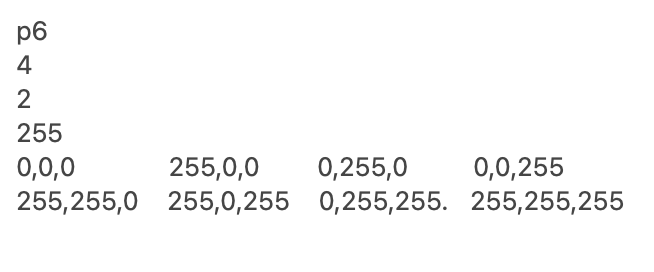
\includegraphics[width=\textwidth]{Bilder/demograph.png}
\caption{ein Beispiel für P6 PPM}
\end{minipage}
\hfill
\begin{minipage}{0.45\textwidth}
\centering

\includegraphics[width=\textwidth]{Bilder/demograph.ppm.png}
\caption{erzeugt durch den Beispielcode}
\end{minipage}
\end{figure}

\par
Die erste Phase des Projekts ist die Graustufenkodierung. Dafür verwenden wir die Formel (1) unten. Dabei wird der gewichtete Durchschnitt der Rot-, Grün- und Blau-Werte jedes Pixels ermittelt. Ein Beispiel der Graustufenkodierung ist in Abbildung 3 zu sehen. 
\begin{equation}
D(x,y) = \frac{a*R+b*G+c*B}{a+b+c}
\end{equation}


\begin{figure}[h]
\centering

\includegraphics[width=0.2\textwidth]{Bilder/gamma1.pgm.png}
\caption{Graustufen Konvertierung von Abb.2}
\end{figure}

\par
Im zweiten Teil der Aufgabe befassen wir uns nun mit einem anderen Aspekt des menschlichen visuellen Systems (HVS) und zwar der Helligkeit \cite{westin2011gammacorrection}. Diese hat einen großen Einfluss darauf, wie natürlich ein Bild auf uns Menschen wirkt. Die Gammakorrektur ändert die Helligkeit bzw. den Kontrast eines Bildes, und hängt von der Wahl des $ \gamma $ Parameters ab. Bei unserem Algorithmus wird die Gammakorrektur durch folgende mathematische Formel (2) bestimmt. Die Werte D'(x,y) ergeben die Intensität der Graustufenkodierung für alle Pixel (x,y). Ein kleinerer Gammawert führt zu einem helleren Bild, während ein größerer Gammawert zu einem dunkleren Bild führt. Bei $\gamma$ = 1 ist die Gammakorrektur entsprechend linear, der übliche $\gamma$ liegt bei 2,2, und bei $\gamma$ = 3 ist das Bild sehr dunkel \cite{cambridgeincolor2020gammacorrection}.

\begin{equation}
D'(x,y) = {\left( \frac{D(x,y)}{255} \right)}^{\gamma}*255
\end{equation}

\par
Um den Effekt der Gammakorrektur zu visualisieren, betrachten wir nochmal die Abb.3. Unterhalb kann man 3 verschiedene „Helligkeits-Versionen“ von Abb.3 vergleichen.

\begin{figure}[h]
\begin{minipage}{0.3\textwidth}
\centering

\includegraphics[width=\textwidth]{Bilder/gamma0.1.pgm.png}
\caption{$\gamma$ = 0.1}
\end{minipage}
\hfill
\begin{minipage}{0.3\textwidth}
\centering

\includegraphics[width=\textwidth]{Bilder/gamma1.pgm.png}
\caption{$\gamma$ = 1}
\end{minipage}
\hfill
\begin{minipage}{0.3\textwidth}
\centering

\includegraphics[width=\textwidth]{Bilder/gamma10.pgm.png}
\caption{$\gamma$ = 10}
\end{minipage}
\end{figure}

\par
Die Hauptfunktion unseres Programms erhält 6 Parameter. Zwei davon sind \texttt{input\_file\_name} und \texttt{output\_file\_name}, welche die Pfade des Eingabebildes und des Ausgabebildes repräsentieren. Der Parameter \texttt{version} vom Datentyp \texttt{int} gibt die Version an. Der Parameter \texttt{benchmark\_number} repräsentiert die Anzahl der Benchmark-Zyklen. Die Parameter \texttt{a}, \texttt{b}, und \texttt{c} vom Datentyp \texttt{float} stellen die RGB-Gewichte für die Graustufenumwandlung dar. Schließlich erhält die Funktion noch einen Parameter \texttt{\_gamma} vom Datentyp \texttt{float}, der für den Gammawert steht.

\par
Obwohl die oben genannten Parameter zusätzlich zu den Ein- und Ausgängen standardmäßig mit sinnvollen Defaultwerten besetzt sind, kann der Nutzer diese Parameter auch selbst mit spezifischen und sinnvollen Werten ersetzen. Wenn die gesetzten Werte nicht sinnvoll sind, wird eine Fehlermeldung ausgegeben und das Programm wird beendet. Hier ist eine Übersicht an Optionen, die der Nutzer beim Aufrufen des Programms setzen kann:

\begin{itemize}
\item Option \emph{-V<Zahl>} --- Die Option -V 0 ist die Standardimplementierung. -V 1 steht für die Implementierung V1 mit Taylorreihe. -V 2 steht für die Implementierung V2 mit SIMD. Andere Werte sind nicht erlaubt.
\item Option \emph{-B<Zahl>} --- Falls gesetzt, wird die Laufzeit der angegebenen Implementierung gemessen und ausgegeben. Das Argument gibt die Anzahl an Wiederholungen des Funktionsaufrufs an. Es darf nicht kleiner als 1000 sein.
\item Positionales Argument \emph{<Dateiname>} --- Der Pfad zur Eingabedatei ist ein obligatorischer Parameter. Falls dieser ungültig ist, wird eine Fehlermeldung ausgegeben und das Programm wird beendet.
\item Option \emph{-o<Dateiname>} --- Der Pfad zur Ausgabedatei ist ein obligatorischer Parameter. Falls dieser ungültig ist, wird eine Fehlermeldung ausgegeben und das Programm wird beendet.
\item Option \emph{-{}-coeffs<FP Zahl>,<FP Zahl>,<FP Zahl>} --- Die drei Argumente müssen stets nicht-negativ sein und dürfen nicht den Wert Infinity und NaN annehmen. Ihre Summe darf auch nicht 0 betragen.
\item Option \emph{-{}-gamma<Floating Point Zahl>} --- Der Gammawert kann nicht negativ sein. Wenn diese Option nicht gesetzt wird, wird standardmäßig der Wert 1 verwendet.
\item Option \emph{-h|-{}-help} --- Eine Beschreibung aller Optionen des Programms und Verwendungsbeispiele werden ausgegeben und das Programm danach beendet. 
\end{itemize}

\section{Lösungsansatz}

\par
Nun wird die Implementierung des Programms betrachtet. Zu Beginn erhält das Programm die Optionen und ihre Argumente von der Eingabe des Nutzers durch die Methode \texttt{getopt\_long} \cite{getoptlong3}. Nach erfolgreichem Einlesen der Eingabe werden alle Argumente auf Korrektheit überprüft. Bei illegalen Argumenten wird das Programm mit einer Fehlermeldung beendet.

\par
Die Versionsnummer der Implementierung kann entweder 0, 1 oder 2 sein. Bei den Versionen 0 und 1 werden lediglich sequenzielle Anweisungen verwendet. Version 2 verwendet wiederum SIMD-Instruktionen zur Berechnung der Graustufenkonvertierung.

\par
In allen aufgerufenen Funktionen wird zunächst die Eingabedatei gelesen. Gemäß der Netpbm-Dateibeschreibung ist eine ppm-Datei in zwei Teile unterteilt: Metadaten und Pixelbereich. Es wird darauf geachtet, dass in den Metadaten ein Kommentar an beliebiger Stelle eingefügt werden kann. Daher wird beim Lesen der Metadaten in der ppm-Datei ein Zustandsautomat entworfen, um alle möglichen Randfälle abzufangen und zu behandeln(siehe Abb. 7).

\begin{figure}[h]
    \centering
    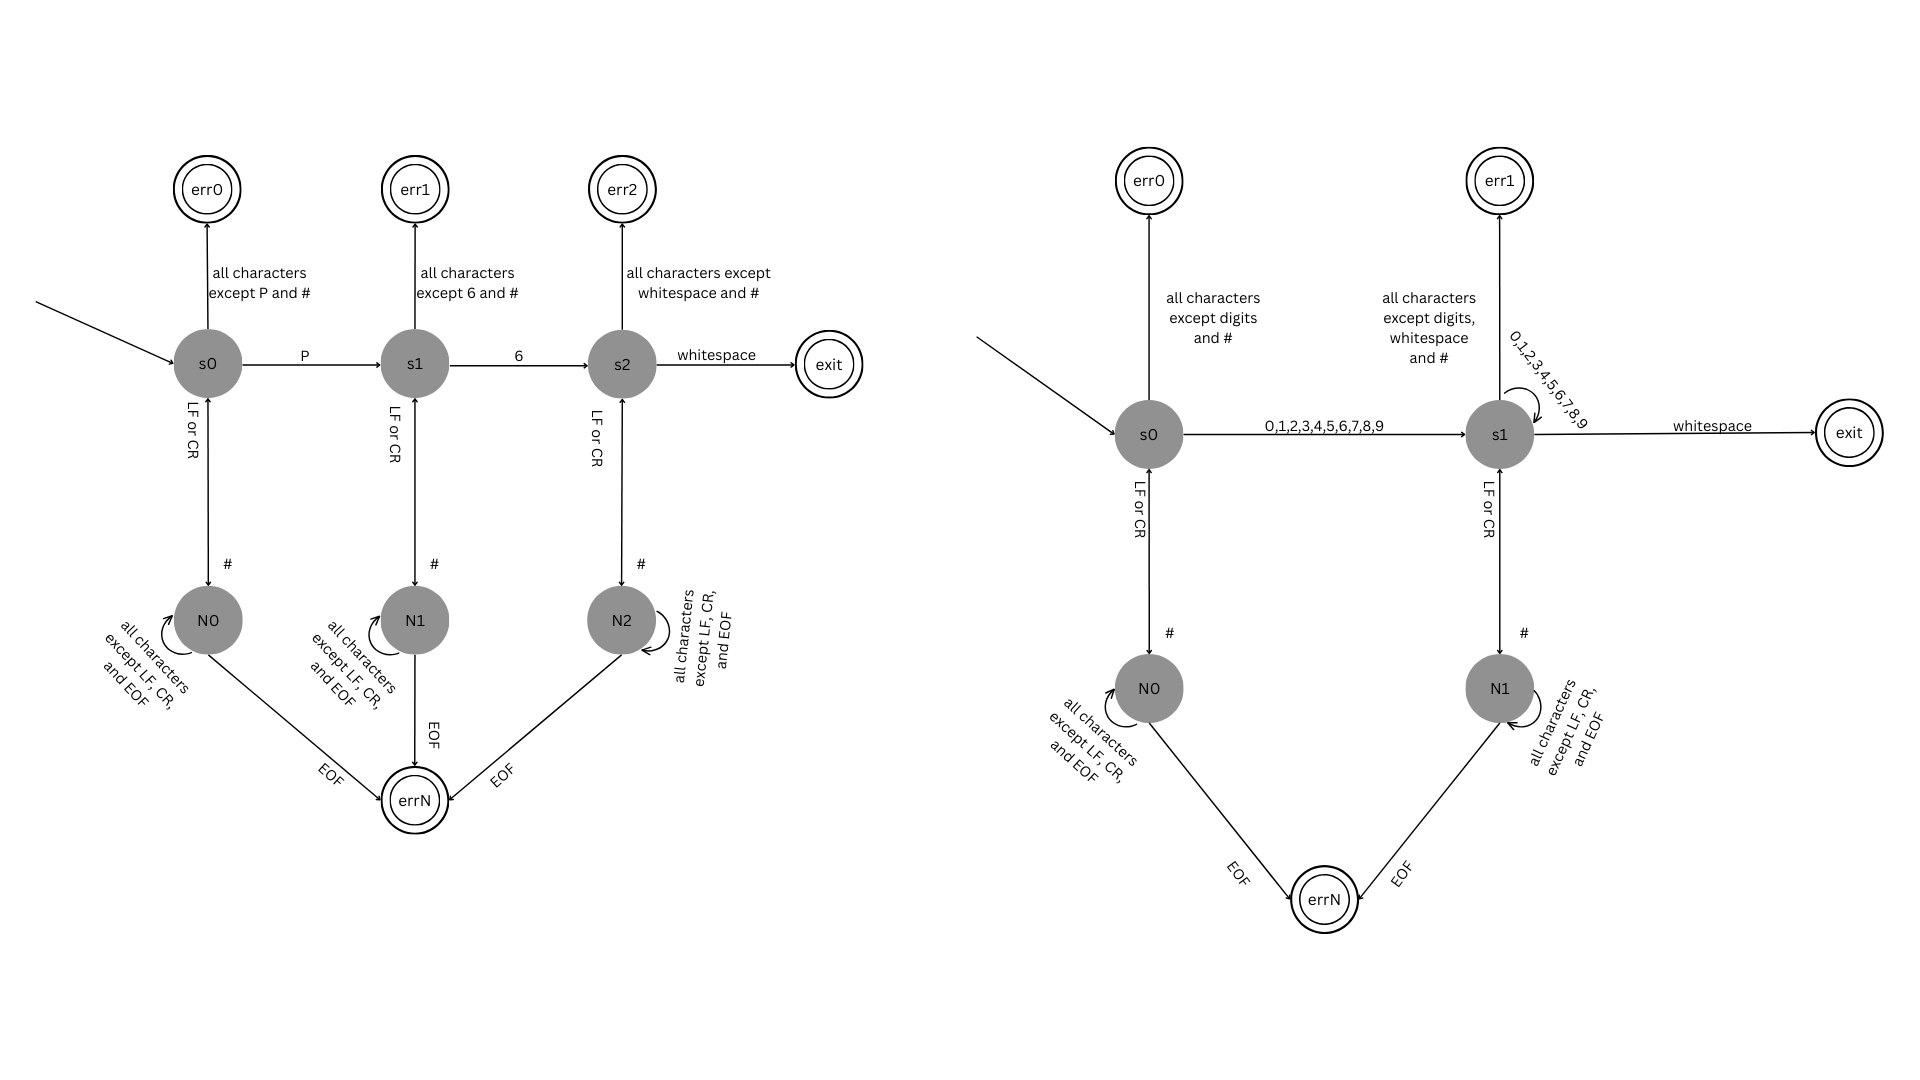
\includegraphics[width=0.9\textwidth]{Bilder/auto.png}
    \caption{Zustandsautomat für das Lesen der Metadaten in der ppm-Datei}
\end{figure}

\par
Der Speicher für die Eingabedaten und Ausgabedaten wird basierend auf den Metadaten der Eingabedatei allokiert. Bei der Implementierung von V0 und V1 werden die drei Farben jedes Pixels beim Lesen der Eingabedatei in der originalen Reihenfolge gespeichert. Bei der Implementierung von V2 werden beim Einlesen die drei Farben jedes Pixels getrennt gespeichert. Deshalb werden drei Speicherbereiche im Heap erstellt, die jeweils für eine bestimmte Farbe alle Pixel-Werte in fortlaufender Reihenfolge speichern. In der \texttt{main}-Funktion wird eine Switch-Anweisung verwendet, um verschiedene Funktionen gemäß der gewählten Versionen aufzurufen.

\par
In V2, der SIMD-Implementierung, wird \texttt{aligned\_alloc} \cite{man2022aligned_alloc} verwendet, um Speicher zu reservieren. Die Startadresse des Speichers wird auf ein Vielfaches von 16 ausgerichtet und erhöht damit die Geschwindigkeit des Ladens und Zurückschreibens von und aus dem Speicher in die xmm-Register. Anschließend wird die ausgewählte Version von \texttt{gamma\_correct} aufgerufen. In V0 und V1 wird die Graustufenkonvertierung für jeden Pixel sequentiell berechnet. V2 verwendet SIMD-Anweisungen, welche es ermöglichen die Graustufenwerte von vier Pixeln gleichzeitig zu berechnen. Hier noch eine Bemerkung: Wir setzen die Standardwerte von a, b, c wie folgt fest: a = 0.299 b = 0.587 c = 0.114. Diese Gewichtungen werden häufig verwendet \cite{w3c1996sRGB}, da sie in der Praxis gute Ergebnisse liefern und die Luminanzeigenschaften der Farben somit natürlich für das menschliche Auge wirken. Nachdem die Graustufenwerte der Pixel berechnet wurden, verwenden V0 und V2 die \texttt{pow}-Funktion der \texttt{math.h} Bibliothek, um die Graustufenwerte nach der Gammakorrektur für jedes Pixel sequentiell zu berechnen. V1 verwendet keine Bibliotheksfunktionen. Im nächsten Teil werden wir sehen, wie V1 grundlegende mathematische Operationen verwendet um die \texttt{pow}-Funktion durch die Taylor-Entwicklung zu approximieren.

\par
Die Taylor Entwicklung \cite{mathworld2024taylorseries} dient der lokalen Approximation eines Funktionswertes und hat die allgemeine Form $f(x) = f(a) + f'(a)(x-a) + \frac{{f''(a)(x-a)^2}}{2!} + \frac{{f'''(a)(x-a)^3}}{3!} + \ldots + \frac{{f^n(a)(x-a)^n}}{n!} + R_n(x) $. Wir verwenden den Fall $a = 1$ und erhalten dann folgende Formel:

\begin{equation}
f(x) = 1 + \frac{(x-1)^1}{1!} (\gamma) + \frac{(x-1)^2}{2!} (\gamma)(\gamma-1)  + \cdots + \frac{(x-1)^n}{n!} \prod_{i=0}^{n-1} (\gamma-i) + R_n(x)
\end{equation}

\par
Im Folgenden bezieht sich Basis immer auf $\frac{D(x, y)}{255}$. Betrachten wir zunächst drei mögliche Grenzfälle. 
\begin{enumerate}
\item Wenn die Basis kleiner oder gleich \(0.5\) ist und $\gamma$ größer oder gleich \(150\) ist, ist das Ergebnis immer \(0\) (\textbf{Underflow} für \texttt{float}).
\item Wenn die Basis \(1.0\) beträgt, ist das Ergebnis immer \(1\).
\item Wenn $\gamma$ größer ist als die magische Zahl \(75464577\),  ist das Zwischenergebnis kleiner als 0,5 und muss nach dem Runden des endgültigen ppm-Wert 0 sein für alle positive Basis kleiner als 1.
\end{enumerate}

\par
Eine weitere Beobachtung für Formel (2) ist, dass die Basis immer eine Zahl zwischen 0 und 1 ist. {$\gamma$} ist laut Angabe so zu wählen, dass es größer als 0 und nicht \emph{Infinity} oder \emph{NaN} ist. Bei der Entwicklung haben wir festgestellt, dass die Berechnung von \(\prod_{i=0}^{n-1} (\gamma-i)\) bei größeren Gammawerten leicht zu einem \textbf{Overflow} führt. Um dieses Problem zu lösen, zerlegt V2 den Gammawert in eine ganze Zahl und eine Dezimalzahl und berechnet diese separat.

\par
Für den Ganzzahlanteil ist unser Designgedanke, den Exponenten in eine binäre Zahl umzuwandeln und dann zu zerlegen. Im folgenden Beispiel wird die 29. Potenz von 0,79 berechnet.

\[
29 = 1 \cdot 2^0 + 0 \cdot 2^1 + 1 \cdot 2^2 + 1 \cdot 2^3 + 1 \cdot 2^4
\]
\[
0.79^{29} = 0.79^{2^0} \cdot 0.79^{2^2} \cdot 0.79^{2^3} \cdot 0.79^{2^4}
\]

\par
Da $\gamma$ kleiner als die magische Zahl 75464577 ist, also zwischen $2^{26}$ und $2^{27}$ liegt, benötigen wir unabhängig vom Exponenten höchstens 27 Schleifen.

\par
Danach verwenden wir Formel (3) für den Dezimal-Anteil, und die Akkumulation endet, sobald das Reihenglied klein genug ist. Hier ist zu beachten, dass wir das Ergebnis des i-ten Reihengliedes zur Berechnung des (i+1)-ten Reihengliedes verwenden können.

\par
Die Graustufenwerte nach der Gammakorrektur werden über einen weiteren Funktionsaufruf im Format von pgm in die Ausgabedatei geschrieben. PGM (Portable Gray Map) Format \cite{netpbm} wird zur Speicherung von Graustufenbildern verwendet, weil es ein einfaches, leicht umsetzbares Bildformat ist. Im Vergleich zu anderen komplexen Bilddateiformaten ist das pgm-Format sehr einfach. Es speichert die Pixelwerte des Bildes und kann leicht in Textform bearbeitet und gelesen werden. Dieses Format erfordert keine komplizierten Dekodierer oder zusätzliche Datenkompression, was es ideal für die schnelle Speicherung und Verarbeitung von Graustufenbilddaten macht. Bevor alle Ressourcen freigegeben werden, wird \texttt{gamma\_correct} wiederholt ausgeführt, wenn der Benutzer die Option \texttt{-B} in den Optionen aktiviert hat. Die Zeit wird zu Beginn und am Ende des Zyklus aufgezeichnet. Diese Laufzeit des Zyklus wird später für die Leistungsanalyse verwendet.

\par
Am Ende des Programms müssen alle Ressourcen freigegeben werden. Zusätzlich wird an sämtlichen Stellen im Programm, an denen eine Allocation oder eine IO-Operation durchgeführt wird, überprüft, ob sie erfolgreich war.

\par
Das Programm verteilt alle Funktionen sinnvoll auf die verschiedenen Funktionen. Jede Funktion ist angemessen groß, logisch korrekt, leicht zu warten und vermeidet Blob Muster.

\section{Genauigkeit}

\par
In diesem Teil der Ausarbeitung beschäftigen wir uns mit der Genauigkeit unserer Implementierung. Um die Genauigkei des gesamten Verfahrens zu studieren, untersuchen wir die Graustufenkonvertierung und die Gammakorrektur separat. In der Phase der Graustufenkonvertierung werden wir den Unterschied zwischen den Ergebnissen von V0 und der offiziellen netpbm-Funktion \textit{ppmtopgm} untersuchen, und in der Phase der Gammakorrektur analysieren wir sie unter dem Gesichtspunkt der mathematischen Konvergenz, bzw. unter dem Gesichtspunkt des realen Fehlers des Programmlaufs.

\par
Zuerst vergleichen wir die Ergebnisse unserer Implementierung mit den Ergebnissen, welche durch das netpbm-Paket generiert wurden. Die Funktion \textit{ppmtopgm} aus dem netpbm-Paket verwendet immer Default-Werte für die Koeffizienten a,b,c, um ein ppm-Bild in ein pgm-Bild zu konvertieren und führt keine direkte Gammakorrektur durch. Daher rufen wir für die Graustufenkonvertierung die Funktion \textit{gamma\_correct} auf und übergeben ihr die Default-Werte für a,b,c und setzten den Gammawert gleich 1. Daraufhin vergleichen wir den prozentualen Unterschied in der Ausgabe und den Wert der insgesamten Differenz für alle möglichen 24bpp-Pixel der beiden Ergebnisse (unsere Implementierung und \textit{ppmtopgm}). Betrachtet man alle mögliche Eingabepixel (($2^{24}$) bzw. 16777216) so zeigt der Vergleich, dass es 8363407 Fälle gibt, in denen das Ergebnis unserer Implementierung in einem Pixel um 1 größer ist als das \textit{ppmtopgm} Ergebnis. Es gibt keine Fälle, bei denen unser Ergebnis in einem Pixel um 2 oder mehr größer ist und es gibt auch keine Fälle, bei denen unser Ergebnis kleiner ist als das von \textit{ppmtopgm}. Dies dürfte darauf zurückzuführen sein, dass in unserem Programm die Funktion \texttt{roundf} aus der Bibliothek \texttt{math.h} verwendet wird, um das Endergebnis zu runden, indem das nicht ganzzahlige Ergebnis auf die nächstliegende ganze Zahl ausgerichtet wird. Dies führt dazu, dass einige Pixelpunkte nach oben gerundet werden, anstatt nur den Bruchteil abzurunden. Bei der Berechnung der Graustufenumwandlung in V0, V1 und V2 wird derselbe Algorithmus verwendet, so dass sie das gleiche Ergebnis liefern.

\par
Die Genauigkeit der Graustufenkonvertierung ist akzeptabel, nun betrachten wir die Genauigkeit der Gammakorrektur. Schauen wir uns als nächstes die Ungenauigkeit aus der mathematischen Perspektive an, wenn das Programm in Version 1 anstelle von \texttt{pow}-Funktion die Formel (3) verwendet hätte. Die Ungenauigkeit entsteht dadurch, dass wir lediglich eine beschränkte Anzahl von Gliedern der Taylorreihe berechnen können. Dadurch werden Glieder ab dem (n+1)-ten vernachlässigt, was zu Genauigkeitsverlusten führt. Zur Schätzung der Präzision ziehen wir das \text{Peano'sche Restglied} \cite{mathematiknet2009taylorpolynome} heran.

\[
o\left((Basis-1)^n\right)
\]

\par
Es zeigt sich, dass das Restglied bei einem Wert von Basis nahe 1 schneller konvergiert. Eine präzisere Beschreibung ermöglicht das Lagrange'sche Restglied \cite{biancahoegel2021taylorformel}, insbesondere da der Exponent ein Bruchteil des $\gamma$ ist und wir uns auf Werte zwischen 0 und 1 konzentrieren. Wir setzen einen Anpassungspunkt von 1 ein und vereinfachen die Lagrangesche Restglied wie folgt:

\[
\frac{{\prod_{i=0}^{n} (\gamma - i) \cdot (x-1)^{n+1}}}{{(n+1)!}} \label{eq:gamma_product}
\]

\par
Wir haben zunächst das $\gamma$ oder Basis fixiert und die Auswirkungen der Änderung der anderen Variablen auf die Anzahl der Iterationen analysiert. Die y-Achse bezieht sich auf die Anzahl an Iterationen, die durchgeführt werden müssen damit das nächste Reihenglied so klein wird, dass es nicht mehr als \texttt{float} darstellbar ist. Die Ergebnisse wurden mit der Software Wolframalpha berechnet. Die Schlussfolgerungen sind in den Abbildungen 8 und 9 dargestellt.

\begin{figure}[h]
    \begin{minipage}{\textwidth}
        \centering
        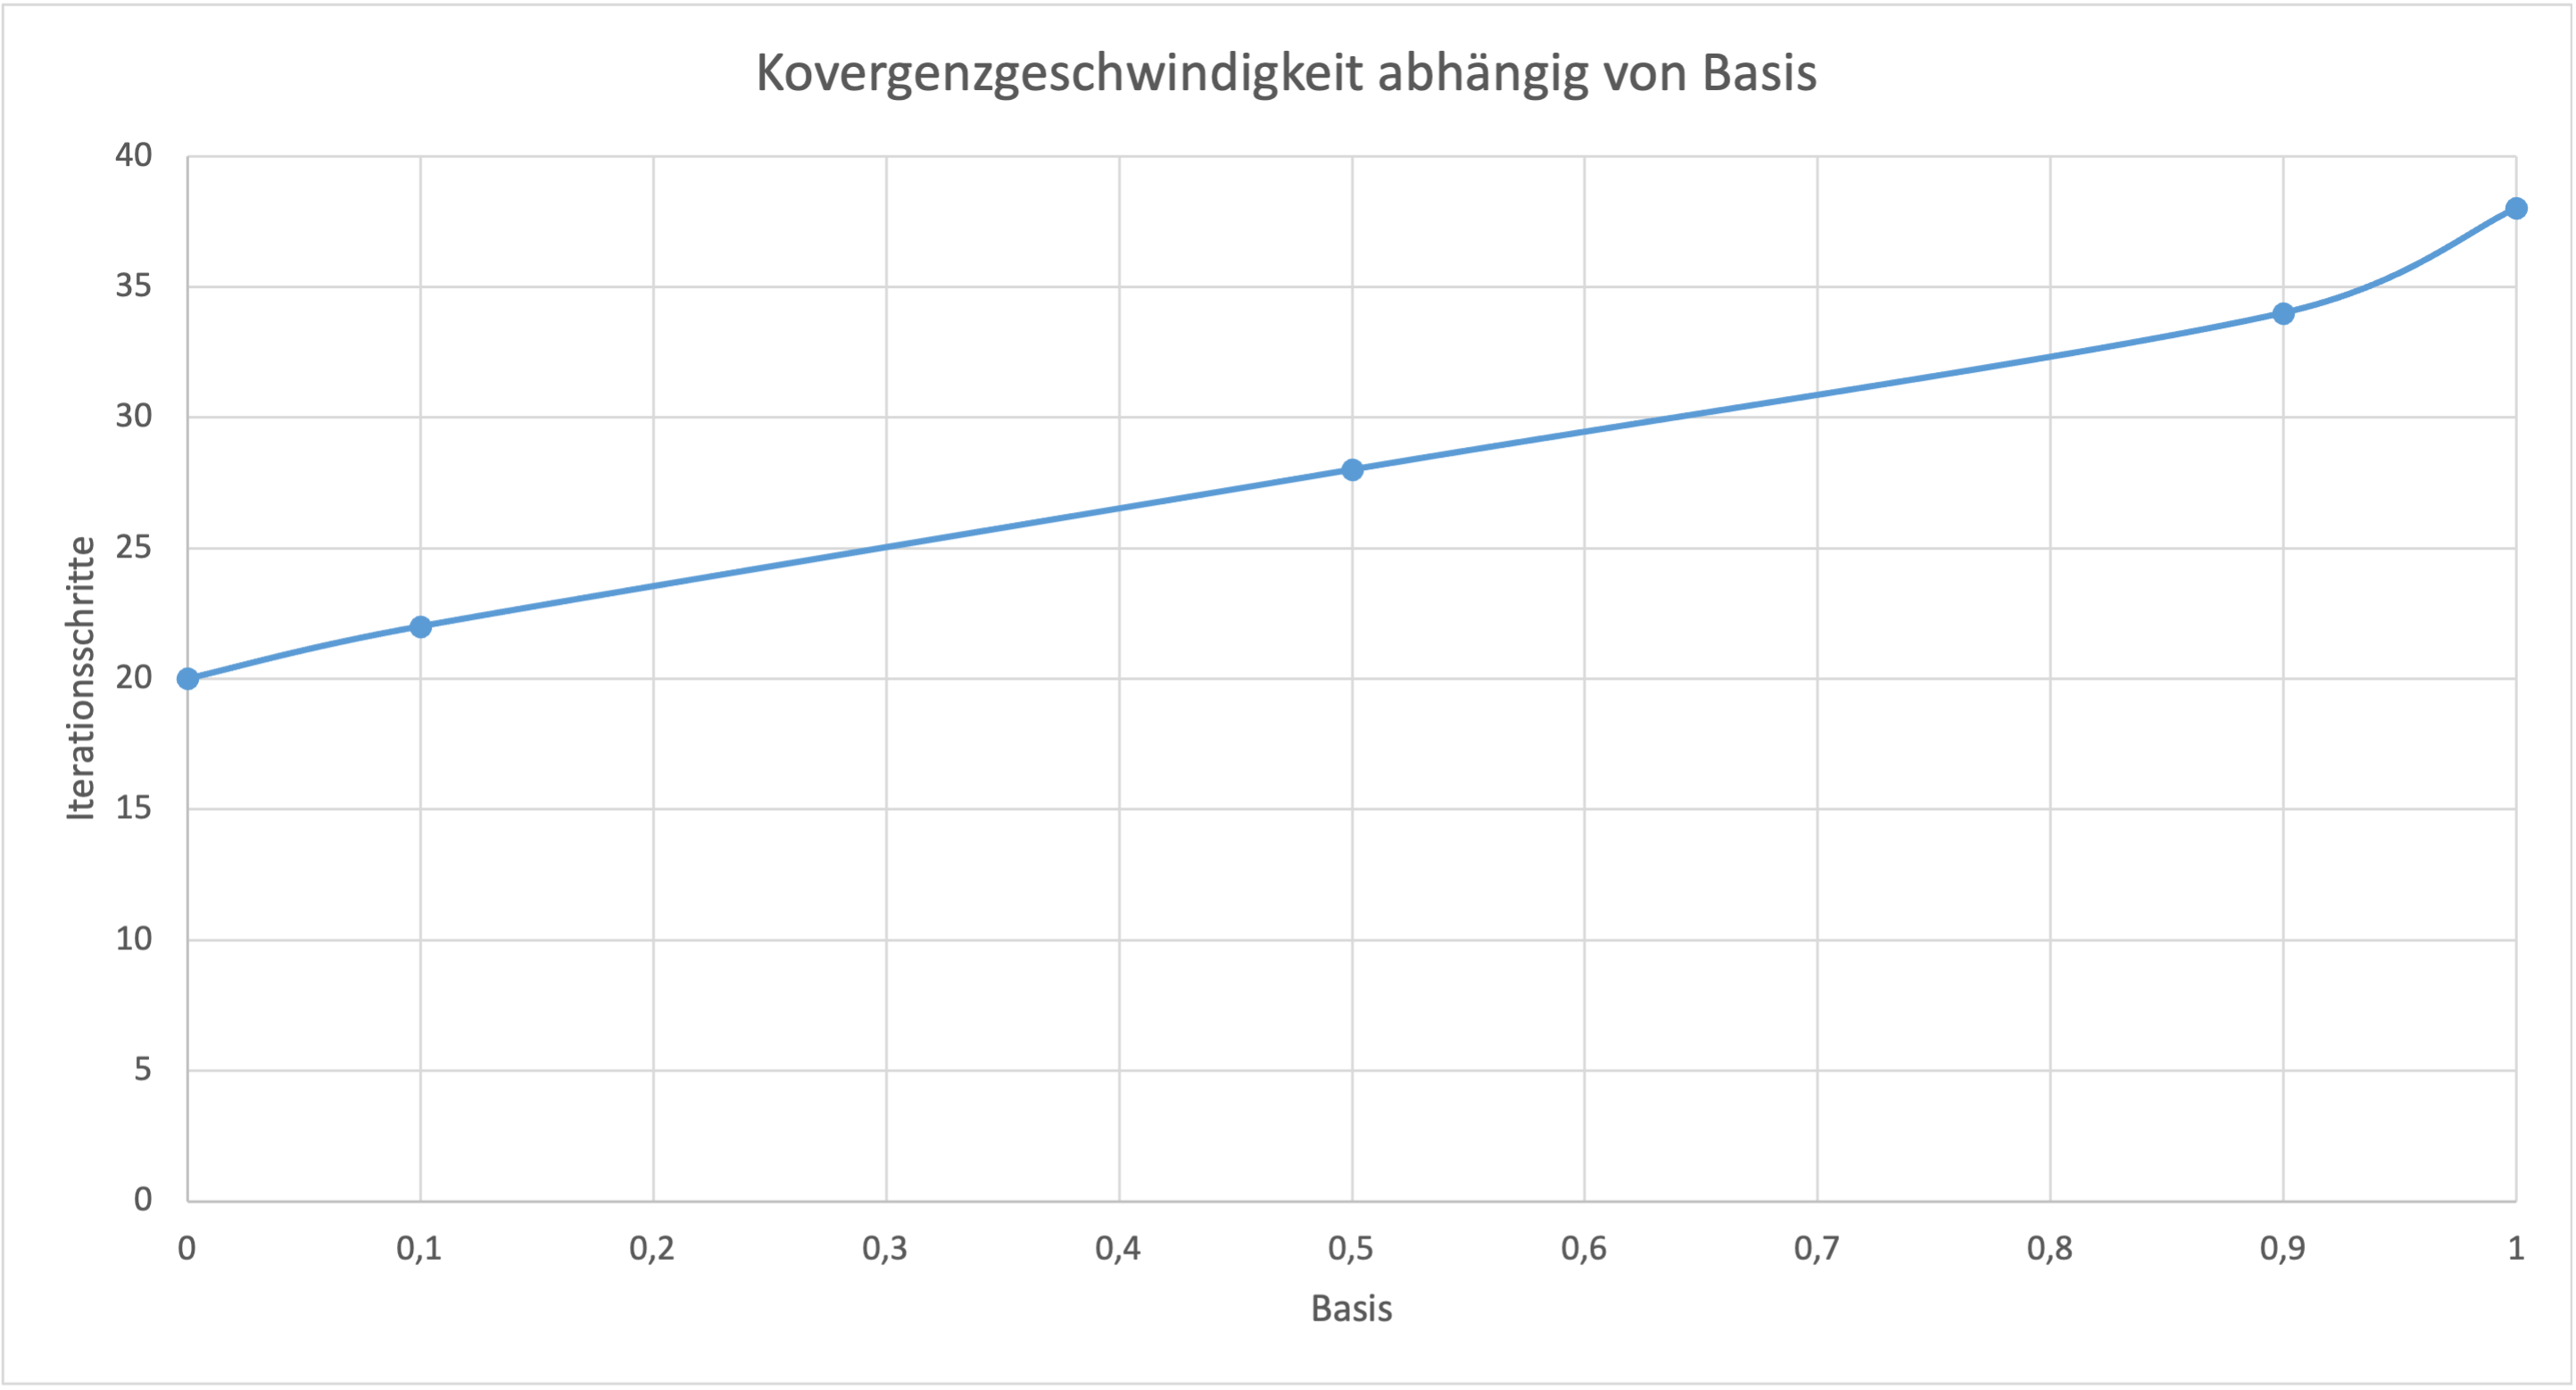
\includegraphics[width=0.65\linewidth]{Bilder/KonvergenzBasis.png}
        \caption{Anzahl der erforderlichen Iterationen für verschiedene x, wenn $\gamma$ auf 0,5 festgelegt ist}
        \label{fig:xchange}
    \end{minipage}
    \begin{minipage}{\textwidth}
        \centering
        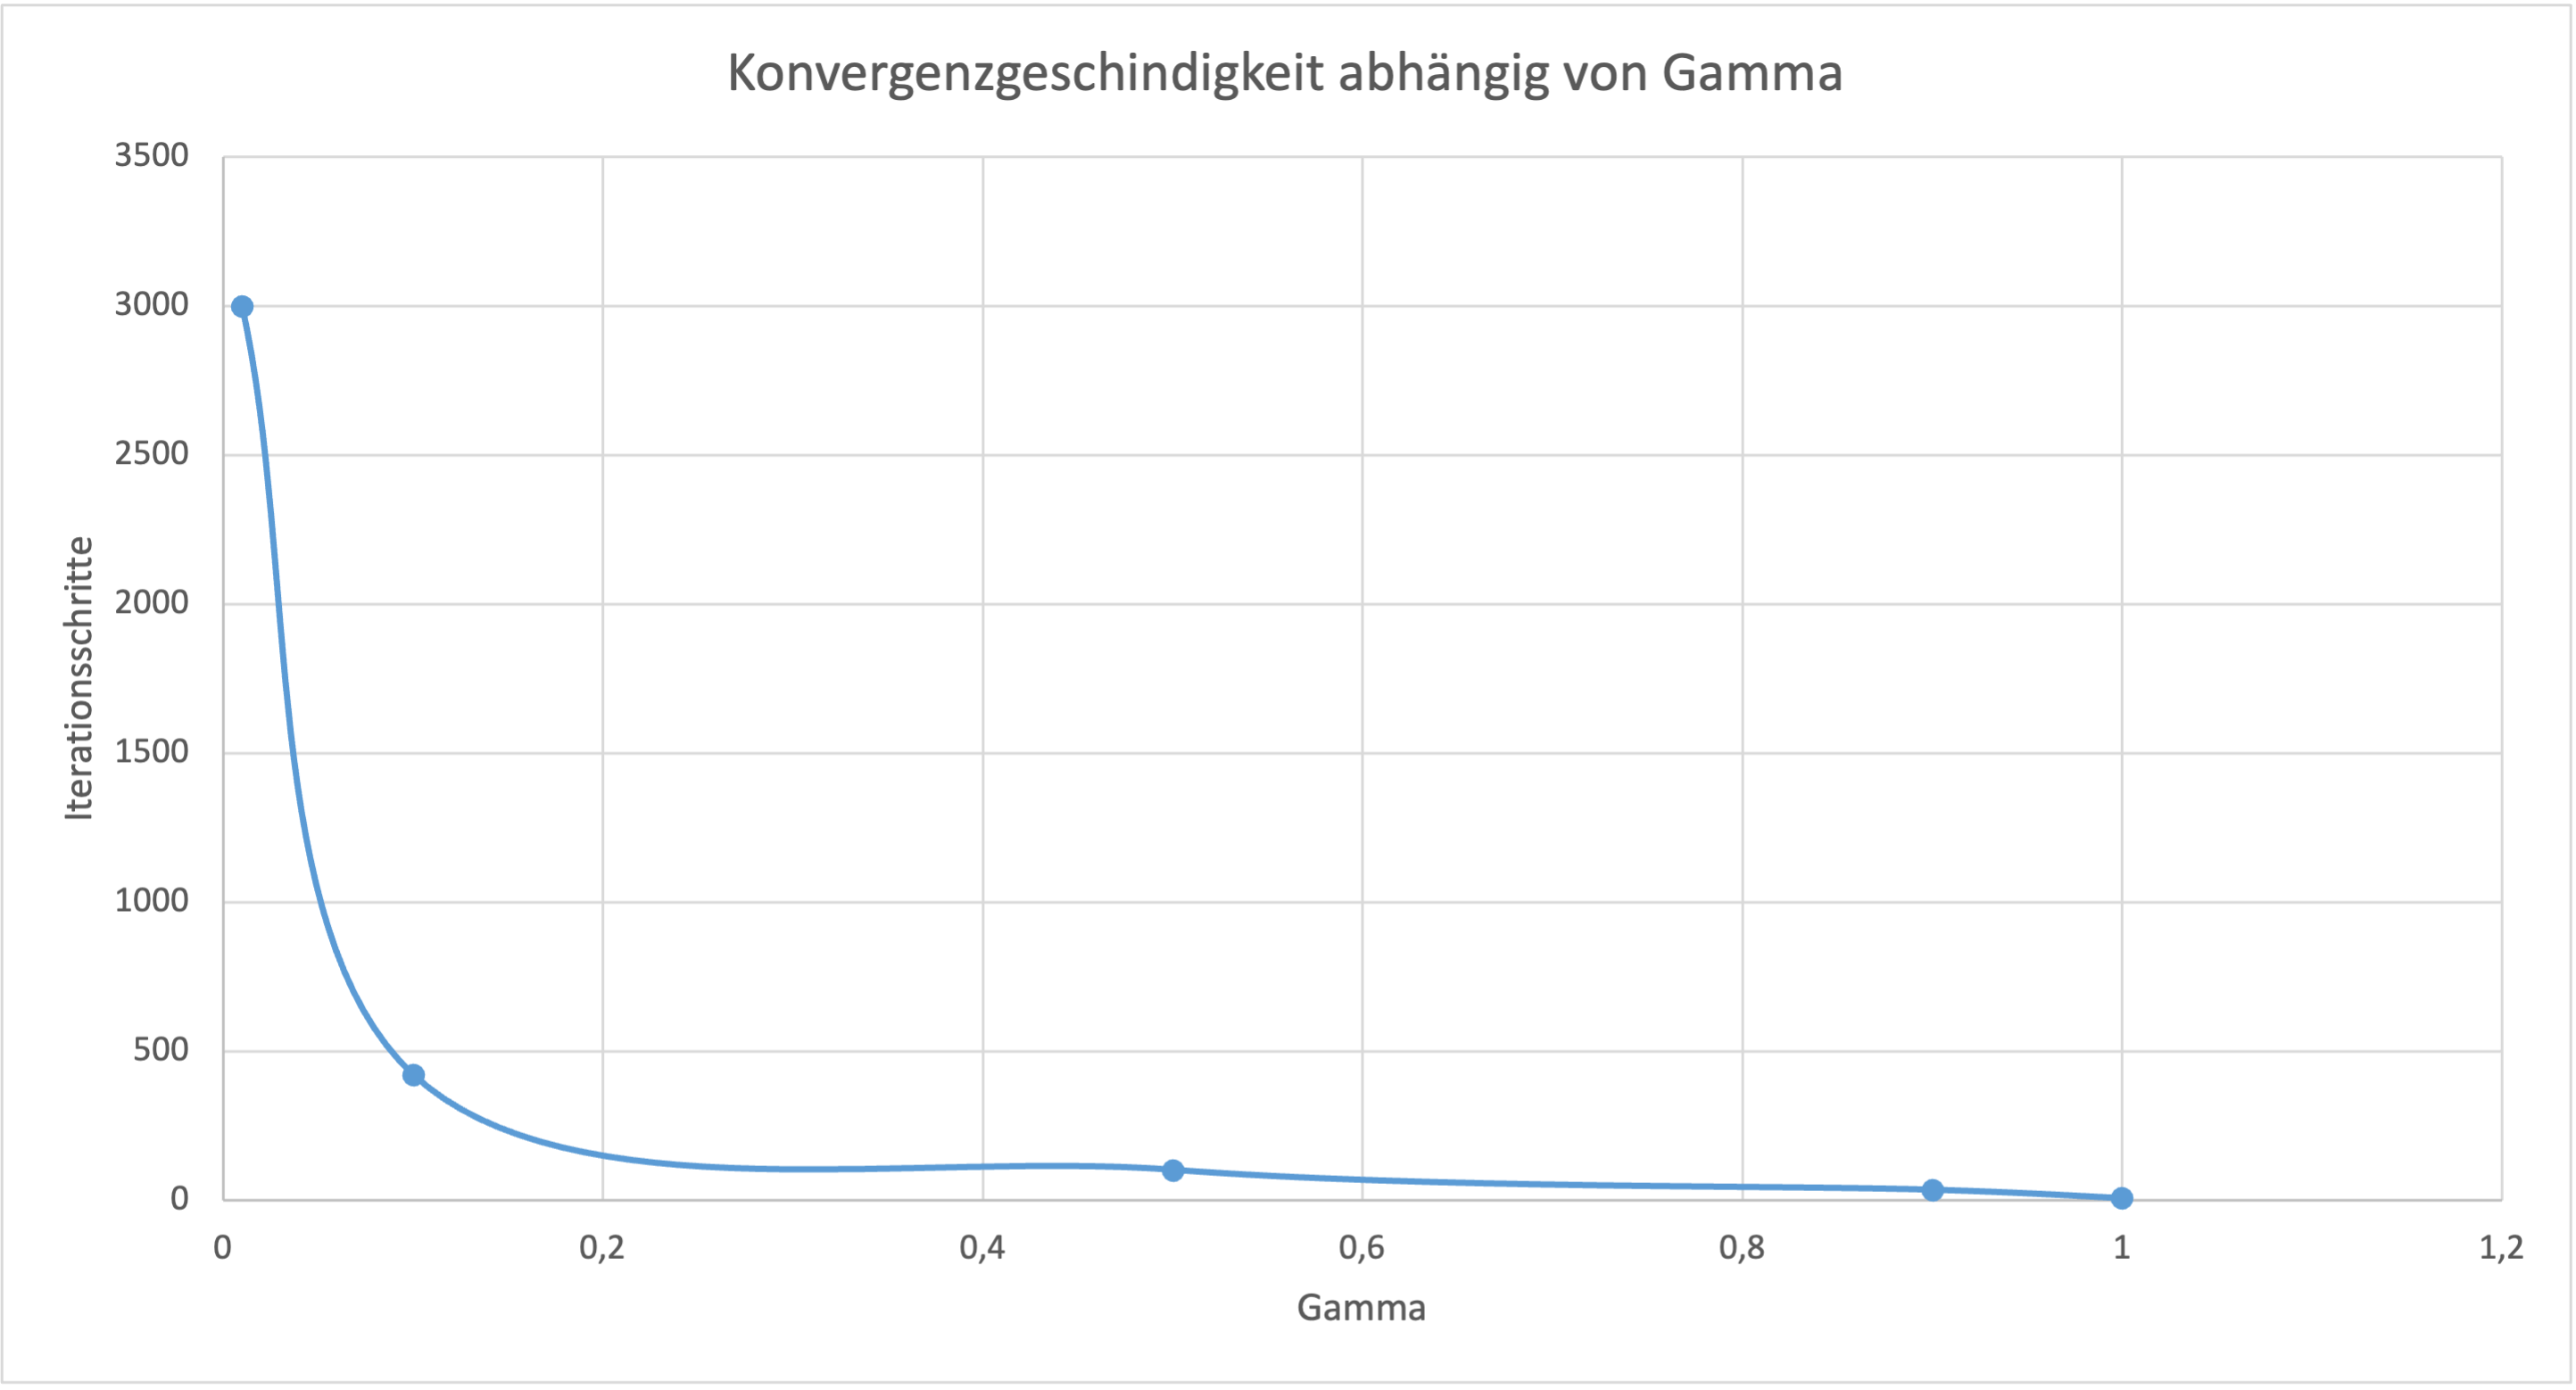
\includegraphics[width=0.65\linewidth]{Bilder/KonvergenzGamma.png}
        \caption{Für verschiedene $\gamma$, wenn x auf 0,9 festgelegt ist}
        \label{fig:gammachange}
    \end{minipage}
\end{figure}

    
\par
Daraus folgt, dass die Auswirkung von $\gamma$ linear und die von der Basis unlinear ist. Wir haben festgestellt, dass bei Basis = 0,0001 sogar mehr als 300.000 Iterationen erforderlich sind. Wenn also die Basis nahe bei Null liegt, wird die Konvergenz langsam sein, was auch zu einem Anstieg des Fehlers führt.

\par
Wir haben eben die Genauigkeit aus einer mathematischen Perspektive heraus geschätzt. Nun betrachten wir den Gesamtfehler, der in unseren Algorithmen durch die Taylorreihe und die Fließkommaoperationen generiert wird. Hierfür haben wir die \texttt{pow}-Funktion als Referenzobjekt gewählt, um die entstandene Abweichung der Funktion \texttt{decimal\_power\_with\_taylor\_expansion} zu analysieren. Die Werte von Basis und Gamma in dieser Funktion liegen im Bereich [0, 1] bzw. [0, 1). Wenn die Abweichung nicht größer als $1/255$ ist, betrachten wir diese Abweichung als akzeptabel, da der Wert eines Pixels in der pgm-Ausagbe dann höchstens um 1 vom Referenzwert abweichen kann. Aus den Ergebnissen des experimentellen Programms schließen wir, dass es nur möglich ist, eine unakzeptable Abweichung für einige der Gammawerte im Wertebereich zu erhalten, wenn die Basis kleiner als $0,000005$ ist (Ergebnis von Basis = 0 ist immer exakt). Bei einer größeren Basis liegt die Abweichung der Ergebnisse immer innerhalb akzeptabler Grenzen, unabhängig vom Wert des Gammas. Aus einer weiteren Analyse lässt sich schließen, dass ein Ergebnis mit einem relativ großen endgültigen Fehler aufgrund einer kleinen Basis ungleich Null nur dann erzielt werden kann, wenn mindestens einer der vom Benutzer eingestellten Koeffizienten a,b,c kleiner als $0,000005$ ist. Eine solche Einstellung ist keine Standardeinstellung für die Koeffizienten und gehört zu keinem der üblicherweise verwendeten Koeffizienten-Werten. Daher befindet sich der Fehler, welcher durch den Algorithmus der Taylorreihe verursacht wird, in akzeptablen Grenzen.

\par
Als Nächstes vergleichen wir den Gamma-Korrekturschritt - wir haben 255 mögliche Graustufen-Pixelwerte, für die wir die V0-, V1- bzw. offizielle netpbm-Methoden verwenden.

\par
Da \textit{pnmgamma} im netpbm-Paket die Ausgabedatei (pgm-Format) nur aus einer pgm-Eingabedatei erzeugen kann, testen wir den Teil der Berechnung der Gammakorrektur in  separat. Da sowohl V0 als auch V2 die \texttt{pow}-Funktion verwenden, sollten sie beide das gleiche Ergebnis liefern. In V1 wird jedoch die Taylorreihe zur Berechnung der Gammakorrektur verwendet, so dass es notwendig ist, die Ergebnisse der beiden Implementierungen mit den Ergebnissen von \textit{pnmgamma} zu vergleichen. Nach dem Vergleich stellt sich heraus, dass für alle möglichen Werte der Graustufen (ganze Zahlen im Bereich von 0-255) und für häufig verwendete Gammawert (von 1 bis 2,2 in 0,1-Schritten) die Ergebnisse beider Algorithmen von \texttt{gamma\_correct} und \texttt{pnmgamma} identisch sind. Deshalb ist die Genauigkeit der Ergebnisse unserer \texttt{gamma\_correct}-Funktion für dieses Problem hoch genug. Da unsere Methode die Graustufen nach der Berechnung der Graustufen in Fließkommazahlen speichert, sollte unser Ansatz theoretisch genauer sein als die zweistufige Berechnung von \textit{ppmtopgm} und \textit{pnmgamma} im netpbm-Paket.

\par
In der Praxis ist die Ungenauigkeit aus den folgenden Gründen relativ gering:
\begin{enumerate}
\item Die Wahrscheinlichkeit für eine Basis kleiner als 0,000005 ist sehr gering.
\item Wenn die Basis klein und gleichzeitig $\gamma$ groß ist, wird dies bereits als Grenzfall berücksichtigt.
\item Wenn das Gammawert einen ganzzahligen Teil enthält, ist das Ergebnis des ganzzahligen Teils kleiner als 1, weil die Basis kleiner als 1 ist. Der absolute Fehler aus dem gebrochenen Teil der Berechnung wird durch Multiplikation reduziert.
\end{enumerate}


\section{Performanzanalyse}
\par
Im vorletzten Teil der Ausarbeitung untersuchen wir nun die Leistung unserer verschiedenen Implementierungen. Dabei analysieren wir bezogen auf die Laufzeit und den Speicherbedarf.

\par
Die theoretische Laufzeit unserer Implementierungen hängt in erster Linie von der Anzahl der Pixel. Die Laufzeit aller 3 Implementationen befindet sich in O(Anzahl-Pixel). Für V0 und V2 werden nur Schleifen zur Bearbeitung des Inputs verwendet. V1 verwendet Schleifen zur Berechnung der Taylorreihe, jedoch ist die Anzahl an möglichen Zyklen in V1 durch eine obere Grenze beschränkt und liegt somit auch in O(Anzahl-Pixel).

\par
Für die praktische Analyse der Laufzeit wurden die 3 Versionen des Algorithmus auf einem Gerät mit folgender Spezifikation evaluiert:

\begin{itemize}
\item Intel Core i5-3337U CPU @ 1.80GHz × 4
\item 16.0 GiB DDR3
\item Ubuntu 22.04.3 LTS 64bit
\end{itemize}

\par
In den zwei Grafiken unten sehen wir das Resultat der Laufzeitanalyse für die 3 verschiedenen Versionen bei unterschiedlichen Benchmarking-Zyklen und unterschiedlichen Gammawerten.

\begin{figure}[h]
\begin{minipage}{0.55\textwidth}
\centering
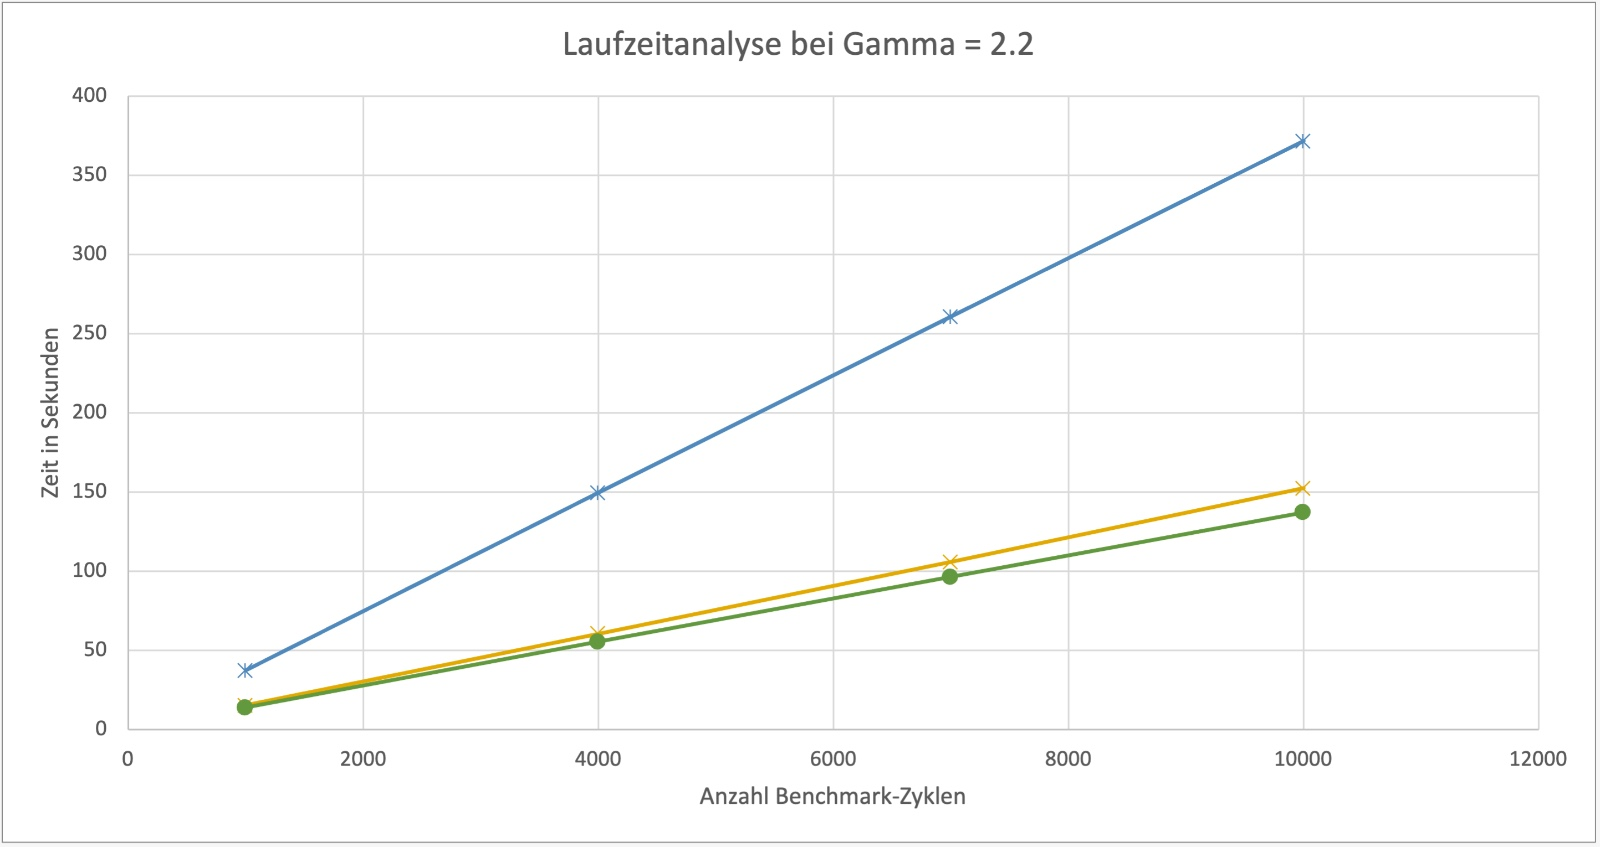
\includegraphics[width=\textwidth]{Bilder/left.jpeg}
\caption{Laufzeit von V0(gelb), V1(blau) und V2(grün)}
\end{minipage}
\hfill
\begin{minipage}{0.55\textwidth}
\centering
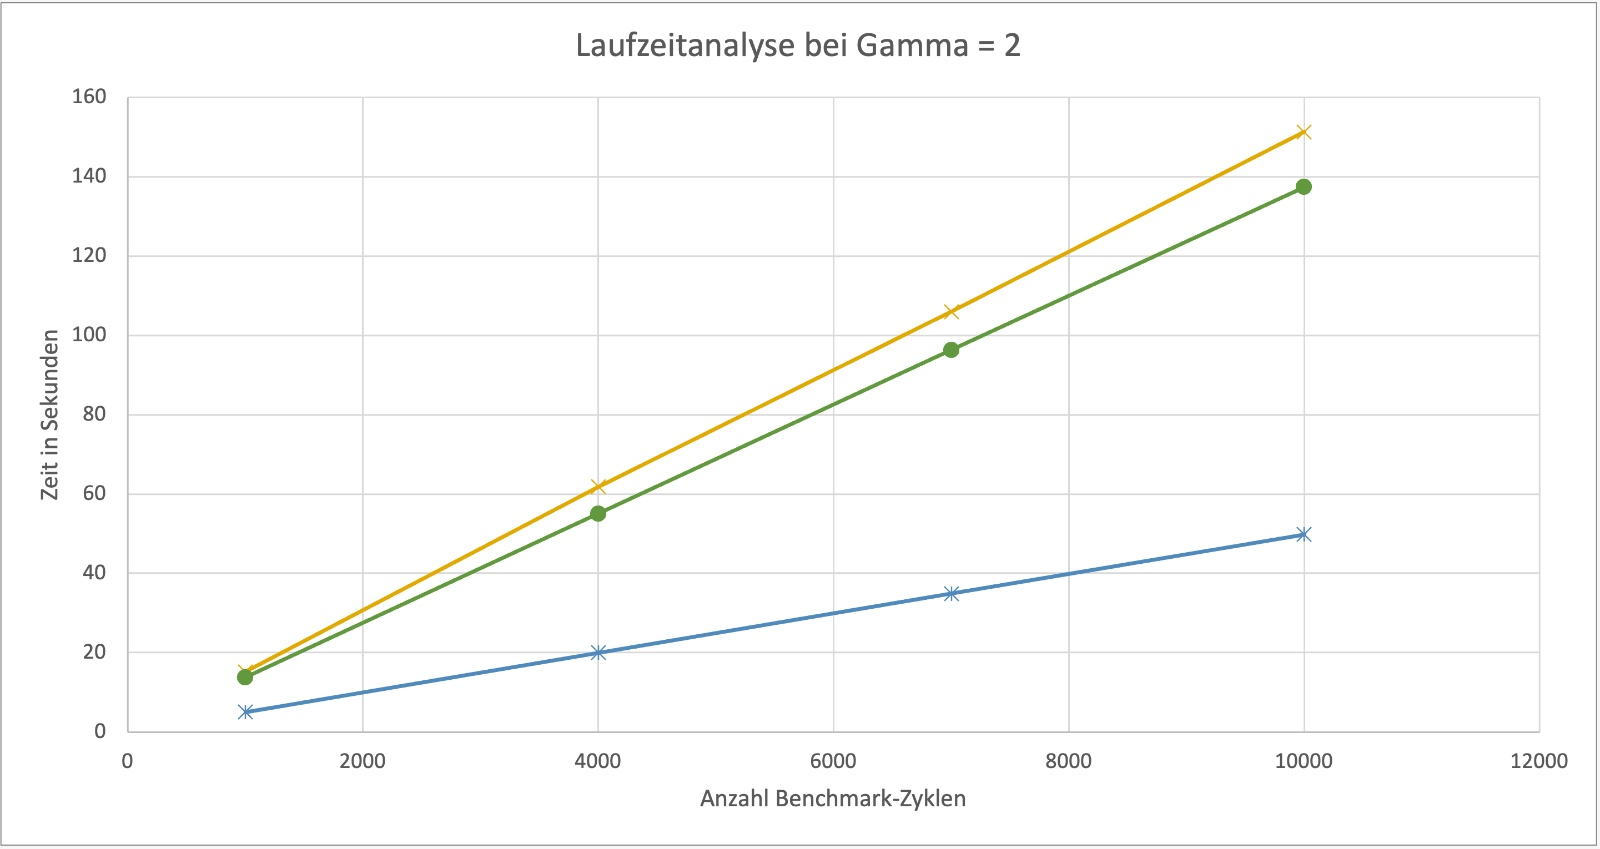
\includegraphics[width=\textwidth]{Bilder/right.jpeg}
\caption{Laufzeit von V0(gelb), V1(blau) und V2(grün)}
\end{minipage}
\end{figure}
    
\par
Die Version 1 ist wie zu erwarten langsamer als Version 0, da sie nicht die \texttt{pow}-Funktion benutzt, sondern selbst die Taylorreihe implementiert. Eine wichitge Ausnahme ist dabei der Fall wo der Gammawert eine ganze Zahl ist (siehe Abb.11). In diesem Fall nimmt unsere Implementationen von V1 einen Shortcut und is somit deutlich schneller als V0/V2. Bei allen anderen Gammawerten ist V0/V2 schneller als V1. 

\par
Durch das Verwenden von SIMD Anweisungen konnte die Laufzeit von V0 etwas verbessert werden.

\par
Bei der Analyse des Speicherbedarfs verwenden wir das Tool “Valgrind”. Dabei handelt es sich um eine Sammlung von Programmierwerkzeugen, die unter anderem die Speichernutzung eines Programms protokollieren kann. Beim Ausführen unseres Programms mit 9 verschiedenen Eingabe-Bildern unterschiedlicher Größe kamen wir zu folgenden Ergebnissen (Abb.12).

\begin{figure}[h]
\centering
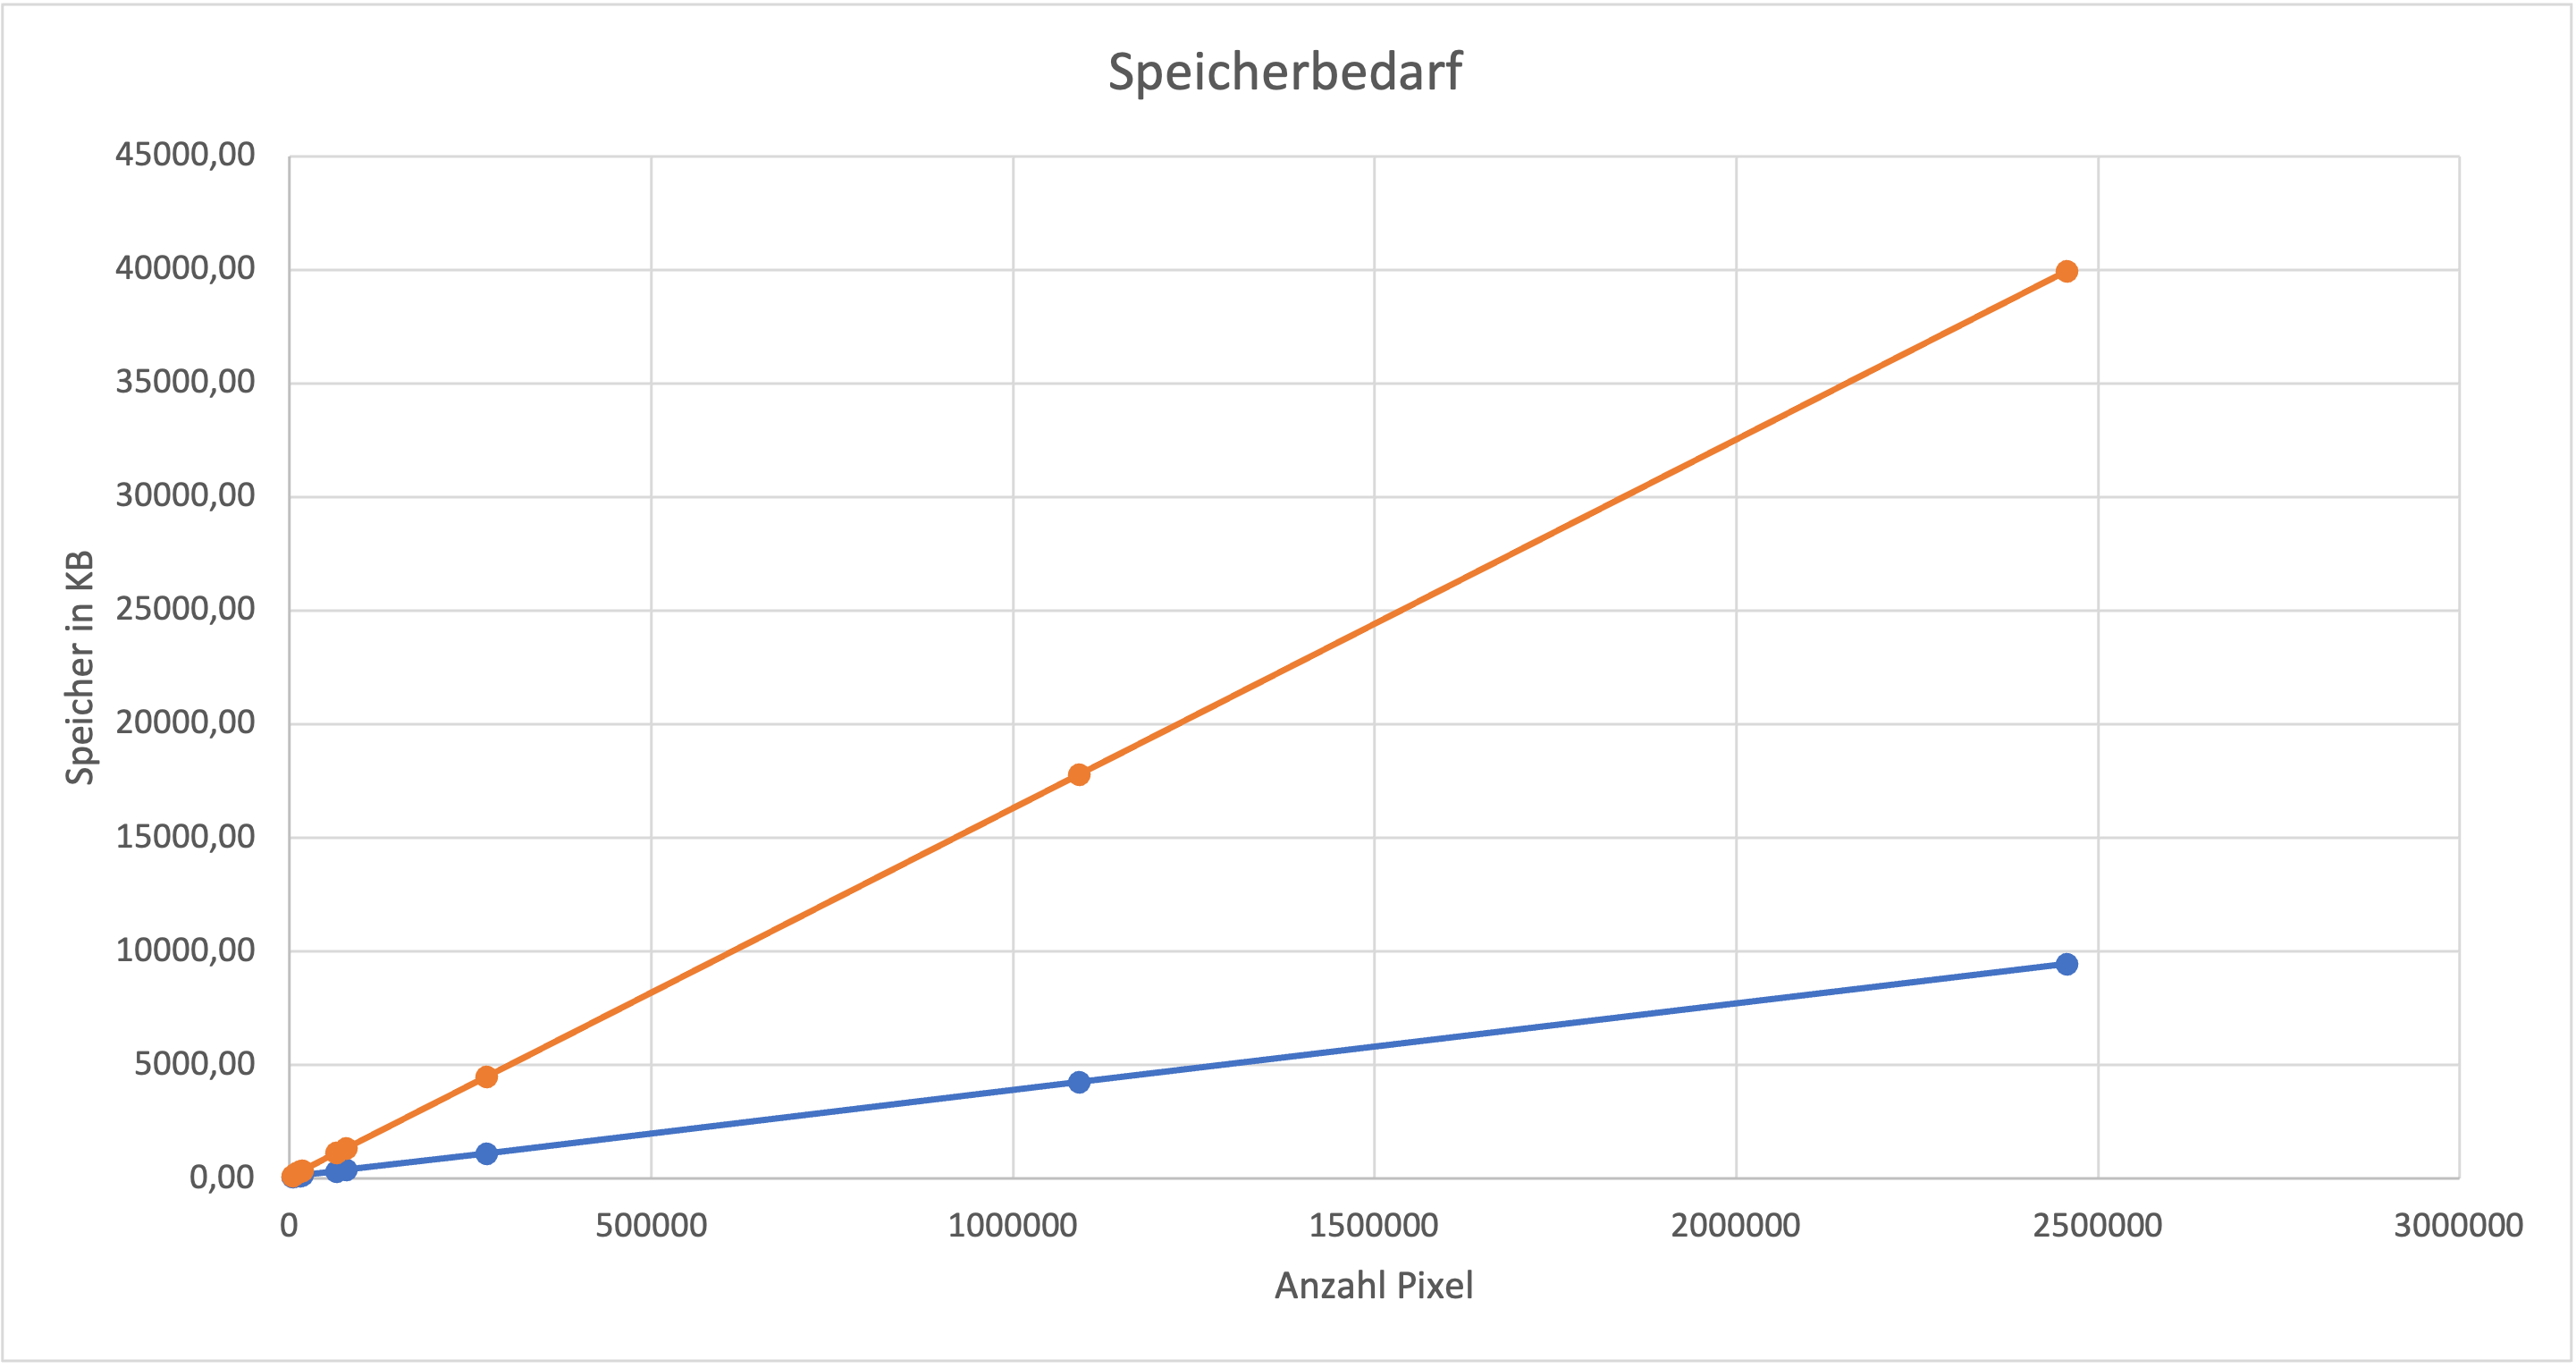
\includegraphics[width=1\textwidth]{Bilder/Speicherbedarf2.png}
\caption{Speicherbedarf für V0/V1 (blau) und V2 (orange)}
\end{figure}

\par
Für alle 3 Implementierungen kann man einen linearen Zusammenhang zwischen Bildgröße und Speichernutzung beobachten. V0 und V1 haben jeweils sehr ähnliche Resultate geliefert, weshalb sie in der Grafik zusammengefasst wurden. Beide Implementationen haben ungefähr eine Speichernutzung von 3,7 KB pro 1000 Pixel. Die Implementierung V2 verbraucht mit 16 KB pro 1000 Pixel im Vergleich deutlich mehr Speicher.

\par
Diese Unterschiede in der Speichernutzung stimmen mit unseren theoretischen Überlegeungen überein. Beim Laden des PPM-Bildes für die SIMD Version werden die \texttt{uint8\_t}-Werte der Pixel als \texttt{float} gespeichert. Dadurch kommt es zu einem 4x größeren Speicherbedarf für Eingabedateien. Zusätzlich wird bei Version 2 ein Zwischenergebnis für die Pixel als \texttt{float} Werte gespeichert. Daher sollte der Speicherbedarf theoretisch insgesamt um den Faktor 4,25 größer sein. 

\section{Zusammenfassung und Ausblick}

\par
Bei diesem Projekt ging es darum, eine Graustufen-Kodierung und Gammakorrektur selber zu programmieren. Das Umsetzen der Graustufen-Kodierung war relativ einfach, genau wie die Implementierung mit der \texttt{pow}-Funktion. Die Aufgabe erhielt eine neue Stufe an Komplexität, sobald es zur Implementierung mit der Taylorreihe und der SIMD Implementierung kommt. Die Taylorreihe führt zu einer geringeren Genauigkeit. Außerdem erörterten wir, wie das Problem einer langsamen Konvergenzgeschwindigkeit bei der Taylorreihe gelöst werden kann. Unsere Lösung ist die Verwendung einer Lookup Table \cite{jungck2011packetC}, in der wir die genaue Berechnung bei kleiner Basis speichern. Die SIMD-Funktion hat zu einer höhere Performanz von etwa 20 Prozent geführt. Abschließend kann man sagen, dass dieses Projekt einen interessanten Einblick in verschiedene Bildformate, das Approximieren mit Hilfe der Taylorreihe und das Optimieren mit Hilfe von SIMD-Intrinsics geliefert hat.


% TODO: Fuegen Sie Ihre Quellen der Datei Ausarbeitung.bib hinzu
% Referenzieren Sie diese dann mit \cite{}.
% Beispiel: CR2 ist ein Register der x86-Architektur~\cite{intel2017man}.
\bibliographystyle{plain}
\bibliography{Ausarbeitung}

\end{document}








